Formulieren Sie einen Test, mit dem die angemessene Vertretung der
Sterne in einem Sack Mailänderli in vier verschiedenen Formen
getestet werden kann.
\medskip

\hbox to\hsize{%
\begin{minipage}{0.7\textwidth}%\raggedright
\begin{teilaufgaben}
\item Wie lautet die Nullhypothese?
\item Welches $\alpha$ wählen Sie?
\item Was zählen Sie bei der Durchführung des Experiments?
\item Wie gross ist $p$?
\item Wie stark muss das Resultat der Zählung vom Erwartungswert abweichen,
damit Sie die Nullhypothese verwerfen?
\end{teilaufgaben}
\end{minipage}
\begin{minipage}{0.3\textwidth}
\begin{center}
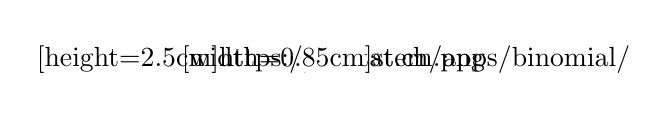
\begin{tikzpicture}[>=latex,thick]
\node at (0,0) {\qrcode[height=2.5cm]{https://wrstat.ch/apps/binomial/}};
\fill[color=white,opacity=1.0] (0,0) circle[radius=0.4];
\node at (0,0) {\includeagraphics[width=0.85cm]{stern.png}};
\end{tikzpicture}
\end{center}
\end{minipage}}

\medskip

\begin{loesung}
\begin{teilaufgaben}
\item Nullhypothese: Die Anzahl der Sterne folgt einer Binomialverteilung mit 
$p=1/\text{Anzahl Formen}$.
\item $\alpha = 0.05$ ist angemessen.
\item Gezählt wird die Anzahl $k$ der Sterne und die Gesamtzahl $n$ der
Mailänderli.
\item $p=\frac14$
\item Es muss getestet werden, ob $k$ um mehr als $\pm1.96\!\sqrt{np(1-p)}$
vom Erwartungswert $np$ abweicht.
Der Faktor $1.96$ ist die 97.5\%-Quantile der Standardnormalverteilung.
\qedhere
\end{teilaufgaben}
\end{loesung}

